\documentclass{standalone}
\usepackage{tikz}
\usepackage{pgfplots}

\pgfplotsset{width=10cm,compat=1.5}

\begin{document}

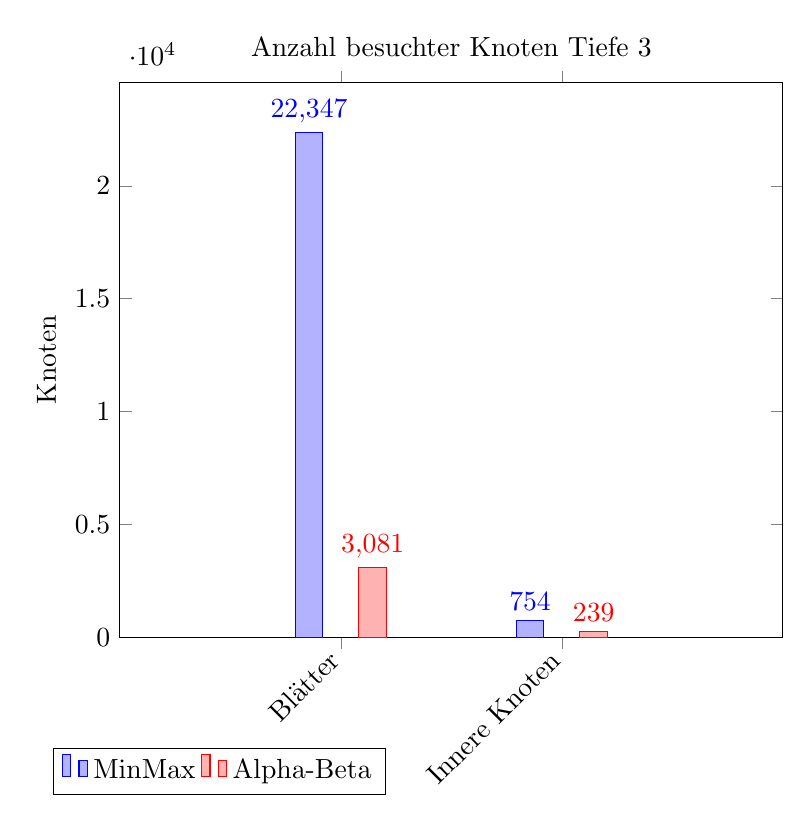
\begin{tikzpicture}
  \begin{axis}[
    title=Anzahl besuchter Knoten Tiefe 3,
    ybar=13pt,
    legend style={at={(0.15,-0.2)},
    anchor=north,
    legend columns=-1},
    ylabel={Knoten},
    ymin = 0,
    symbolic x coords={
      Blätter,
      Innere Knoten
    },
    xtick=data,
    enlarge x limits=1,
    nodes near coords,
    nodes near coords align={vertical},
    x tick label style={rotate=45,anchor=east}
  ]
    \addplot coordinates{
      (Blätter,       22347)
      (Innere Knoten, 754)
    };
    \addplot coordinates{
      (Blätter,       3081)
      (Innere Knoten, 239)
    };
    \legend{
      MinMax,
      Alpha-Beta
    }
  \end{axis}
\end{tikzpicture}


\end{document}